\documentclass{report}

%%%%%%%%%%%%%     PACKAGES     %%%%%%%%%%%%%

\usepackage{marvin} %Custom Package by Marvin Lin
\usepackage{fancyhdr}

%%%%%%%%%%%%%     DOCUMENT FORMATTING     %%%%%%%%%%%%%

\pagestyle{fancy}
\fancyhf{}
\lhead{MTH261 Applied Linear Algebra}
\rhead{Marvin Lin}

\setlength{\parindent}{0pt}

%%%%%%%%%%%%%     TITLE, AUTHOR, ETC.     %%%%%%%%%%%%%

\title{MTH 261 Lecture Notes}
\author{Marvin Lin}
\date{Winter 2022}

%%%%%%%%%%%%%%%%%%%%%%%%%%%%%%%%%%%%%%%%%%%%%%%%%
%%%%%%%%%%%%%     DOCUMENT BODY     %%%%%%%%%%%%%
%%%%%%%%%%%%%%%%%%%%%%%%%%%%%%%%%%%%%%%%%%%%%%%%%

\begin{document}

\maketitle

\tableofcontents

\chapter{Introduction to Linear Algebra}

\section{System of Linear Equations}

Linear Algebra is the area of math concerning liner equations/functions that are represented in vector space and through matrices. If Calculus is the foundational language of mathematics, then Linear Algebra is the foundational language of STEM.

\begin{remark}
Keep in mind that while Linear Algebra utilizes matrices, it is just a tool to solve problems with. The study is \textbf{NOT} of matrices.
\end{remark}

\begin{definition}[Linear Equation]
An equation where $a_1x_1+a_2x_2+\dots+a_nx_n=b$, where $a_1,a_2,a_n, b \in$ as constants of $\mathbb{C}$ and in $\mathbb{R}$
\end{definition}

\begin{definition}[Linear System]
A collection of linear equations with the same variable
\end{definition}

\begin{definition}[Solution \& Solution Set]
A solution satisfies all equations in a system simultaneously, while a solution set is all possible solutions
\end{definition}

\begin{definition}[Equivalent Solutions]
Two systems with the same identical solution set
\end{definition}

\begin{definition}[Types of Solutions]
There are two major classification with solution, which are broken into three major solutions:
\begin{itemize}
	\item Inconsistent (no solutions)
	\item Consistent (at least one solution)
	\begin{itemize}
		\item Unique Solution
		\item Infinite Solutions
	\end{itemize}
\end{itemize}
Since the systems we are exploring and purely linear, there will not be two, three, or more solutions.
\end{definition}
\begin{figure}[h]

\begin{center}
  \includegraphics[width=10cm]{figures/solutions}
  \caption{Types of solutions in a linear system}
  \label{fig:graph1}
\end{center}
\end{figure}

\begin{remark}
This is true for all linear systems in all space
\end{remark}

\begin{definition}[Matrix]
A rectangular array of numbers, often used to compress systems. Let's say the following system of equations is given:
\begin{alignat*}{4}
 x & {}-{} & 7y & {} {} &    {}+{} & 6t & {}={} &  5 \\
   & {} {} &    & {} {} &  z {}-{} & 2t & {}={} & -3 \\
-x & {}+{} & 7y & {}-{} & 4z {}+{} & 2t & {}={} &  7
\end{alignat*}
It can be reduced into the following matrix:
$\begin{bmatrix}
1 & -7 & 0 & 6 \\ 
0 & 0 & 1 & -2 \\ 
-1 & 7 & -4 & 2
\end{bmatrix}$
\end{definition}
\begin{definition}[Augmented Matrix]
A standard matrix which also includes the $\mathbf{b}$ coefficient in the matrix. The following is the augmented matrix of the system of equations from Definition 1.6:
$\begin{bmatrix}
1 & -7 & 0 & 6 \\ 
0 & 0 & 1 & -2 \\ 
-1 & 7 & -4 & 2
\end{bmatrix}
\;OR\;
\begin{bmatrix}
1 & -7 & 0 &\bigm| & 6 \\ 
0 & 0 & 1 &\bigm| & -2 \\ 
-1 & 7 & -4 &\bigm| & 2
\end{bmatrix}$
\end{definition}
\begin{definition}[Elementary Row Operations]
Elementary row operations are used to change matrices in a \underline{revertible} manner.
	\begin{enumerate}
		\item \textbf{Replacement.} Sum of itself and a multiple of another row.
		\item \textbf{Interchange.} Swap/Interchange two rows.
		\item \textbf{Scaling.} Multiply all entries in a row by a nonzero constant.
	\end{enumerate}
\end{definition}

These operations can be used with any matrix, and are typically used to create variations of the matrix that is beneficial to finding specific information.

\begin{definition}[Row Equivilance]
	Matrices are referred to as \underline{row equivilant} if the matrices can be transformed into each other through elementary row operations.
\end{definition}

\subsection*{Existence and Uniqueness}
In analyzing a linear system, a few key questions are being asked:
\begin{enumerate}
	\item Is the system consistent or inconsistent? (Solution or no solution)
	\item Is the solution unique (one solution or many)?
\end{enumerate}
\begin{remark}
	Keep in mind, since we are looking into linear systems, there may only be one solution or infinite solutions, none in between.
\end{remark}
\section{Row Reduction and Echelon Forms}

There are specific forms in which a matrix can be in to provide valuable information about the matrices.
\begin{definition}[Leading Entry]
	The leftmost nonzero entry in a nonzero row.
\end{definition}
In the case of the matrix below, $x$ is the leading entry:
\begin{center}
	$\begin{bmatrix}
		\underline{x} & 2 & 0 & 5
	\end{bmatrix}$	
\end{center}
\begin{definition}[Echelon Form (REF)]
	One of the primary forms, refereed to as row echelon form (often just called echelon form) has the following properties:
	\begin{itemize}
		\item All nonzero rows are above any rows of zeros
		\item Each leading entry is in a column to the right of the leading entry above it
		\item All entries in a column below a leading entry are zeros
	\end{itemize}
\end{definition}
Below is an example of a matrix in Echelon Form (REF):
\begin{center}
	$\begin{bmatrix}
	\underline{4} & 0 & 4 & 3 \\
	0 & \underline{3} & 6 & 1 \\
	0 & 0 & \underline{1} & 8 
	\end{bmatrix}$
\end{center}
The underlined numbers indicate the leading entries.
\begin{definition}[Reduced Echelon Form (RREF)]
	Similar to REF, the reduced echelon form (RREF) takes the definition of the REF a few steps further
	\begin{itemize}
		\item The leading entries are 1
		\item Te leading entry (1) is the only nonzero entry in its column
	\end{itemize}
\end{definition}
Below is an example of a matrix in Echelon Form (REF):
\begin{center}
	$\begin{bmatrix}
	\underline{1} & 0 & 0 & 3 \\
	0 & \underline{1} & 0 & 1 \\
	0 & 0 & \underline{1} & 8 
	\end{bmatrix}$
\end{center}
\begin{theorem}[Uniqueness of RREF]
	Each matrix is only row equivalent to a single RREF matrix.
\end{theorem}
This is ONLY true for RREF. REF can be adjusted with row operations to have multiple matrices.

\subsection*{Pivots}
\begin{definition}[Pivot Positions and Columns]
	Leading entries in REF and the leading 1's in RREF are referred to a \underline{pivot position}. Similarly, a column containing a pivot position is referred to as a \underline{pivot column}.
\end{definition}
These pivots can be identified in the original matrix, and are not terms exclusively for REF and RREF (unlike leading entries).

\subsection*{Gauss-Jordan Elimination}

\begin{fullindent}{1cm}
	\textbf{Step 1.} The leftmost non-zero column must be a pivot column, with the first row in the column being the pivot position.
	\begin{center}
		$A = \begin{bmatrix}
			0 & 4 & 4 & 3 \\
			4 & 4 & 6 & 1 \\
			2 & 0 & 4 & 8
		\end{bmatrix}$
	\end{center}	
	\textbf{Step 2.} Any nonzero entry in the pivot column can be a pivot. Use the interchange ERO to make it the first column.
	\begin{center}
		$\sim \begin{bmatrix}
			2 & 0 & 4 & 8 \\
			4 & 4 & 6 & 1 \\
			0 & 4 & 4 & 3
		\end{bmatrix}$
	\end{center}
	\textbf{Step 3.} Use EROs to make all positions below pivot into zeros.
	\begin{center}
		$\sim \begin{bmatrix}
			2 & 0 & 4 & 8 \\
			0 & 4 & -2 & -15 \\
			0 & 4 & 4 & 3
		\end{bmatrix}$
	\end{center}
	\textbf{Step 4.} Ignore the pivot row and repeat for all remaining rows (ad terminum; until completion/termination).
	\begin{center}
		$\sim \begin{bmatrix}
			2 & 0 & 4 & 8 \\
			0 & 4 & -2 & -15 \\
			0 & 0 & 6 & 18
		\end{bmatrix} = REF(A)$
	\end{center}
\end{fullindent}

This will create a $A \rightarrow REF(A)$, and is common referred to as \textbf{Gaussian Elimination}. The following 2 steps will create $A \rightarrow RREF(A)$ and is referred to as \textbf{Gauss-Jordan Elimination}

\begin{fullindent}{1cm}
	\textbf{Step 5.} Make all pivots 1 through the scaling ERO.
	\begin{center}
		$\sim \begin{bmatrix}
			1 & 0 & 2 & 4 \\
			0 & 1 & -\frac{1}{2} & -3\frac{3}{4} \\
			0 & 0 & 1 & 3
		\end{bmatrix}$
	\end{center}
	\textbf{Step 6.} Begin with the rightmost pivot and use row operations to work upwards, making all entries above pivot positions to be zeros.
	\begin{center}
		$\sim \begin{bmatrix}
			1 & 0 & 0 & -2 \\
			0 & 1 & 0 & -2\frac{1}{4} \\
			0 & 0 & 1 & 3
		\end{bmatrix} = RREF(A)$
	\end{center}
\end{fullindent}

\subsection*{Gauss-Jordan Elimination in Linear Systems}
This method also helps solves linear systems when reduced down to RREF. Assume column 1 is $x_1$, column 2 is $x_2$, column 3 is $x_3$, and column 4 is $b$.
\begin{center}
	$4x_2 + 2x_3 = 3$\\
	$4x_1 + 4x_2 + 6x_3 = 1$\\
	$2x_1 + 4x_3 = 8$
\end{center}

And therefore after applying Gauss-Jordan Elimination is:
\begin{center}
	$\begin{cases}
		x_1 = -2\\
		x_2 = -2\frac{1}{4}\\
		x_3 = 3
	\end{cases}$
\end{center}

In the case of the following where one row is only zeros,
\begin{center}
	$\begin{bmatrix}
		1 & 0 & 0 & -2 \\
		0 & 1 & 0 & -2\frac{1}{4} \\
		0 & 0 & 0 & 0
	\end{bmatrix} = RREF(A)$
\end{center}
we get:
\begin{center}
	$\begin{cases}
		x_1 = -2\\
		x_2 = -2\frac{1}{4}\\
		x_3 = x_3 \rightarrow x_3 \text{ is free}
	\end{cases}$
\end{center}
\begin{definition}
	Variables corresponding with a pivot column is called \textbf{basic variable}, while variables corresponding to a non-pivot column is referred to as a \textbf{free variable}.
\end{definition}
There are three possible definitions of the solution set:
\begin{itemize}
	\item \textbf{No solution.} We write $\phi$ (phi).
	\item \textbf{Unique Solution.} We write the single solution in a set (ie. ${(1, 0, -1)}$).
	\item \textbf{Infinite solutions.} Form a \underline{general solution} by expressing basic variables in terms of the free variable, and notating free variables as free. Also called \underline{parametric solution}, where free variables are the parameters.
\end{itemize}
\begin{theorem}
	The following can be determined by analyzing the augmented matrix:
	\begin{enumerate}
		\item \textbf{A linear system is consistent} if and only if the rightmost column if not a pivot column, in addition to no false statements (ie. $0/neq 1$). \underline{A false statement is a clear indicator of an inconsistent system.}
		\item \textbf{A linear system is consistent and unique} if there are no free variables.
		\item \textbf{A linear system is consistent and has infinite solutions} if there are free variables.
	\end{enumerate}
\end{theorem}
\section{Vector Equations}
\begin{definition}
	Matrix with one column is called column vector, or just a vector.
\end{definition}
\begin{definition}[Equality, Sum, and Scalar]
	A vector is only equal if corresponding entries are equal:
	\begin{center}
		$\begin{bmatrix} 3 \\ 2 \end{bmatrix} \neq \begin{bmatrix} 2 \\ 3 \end{bmatrix}$
	\end{center}
	Vectors can only be added if they are in the same space (ie. $\mathbb{R}^2 vs \mathbb{R}^3$):
	\begin{center}
		$\begin{bmatrix} 3 \\ 2 \end{bmatrix} + \begin{bmatrix} 1 \\ 2 \\ 3 \end{bmatrix} = \text{undefined}$
	\end{center}
	A vector is scaled by multiplying each entry by the scalar, $c$:
	\begin{center}
		$c\mathbf{u} = 4\begin{bmatrix} 3 \\ 2 \end{bmatrix} = \begin{bmatrix} 4(2) \\ 4(3) \end{bmatrix}= \begin{bmatrix} 8 \\ 12 \end{bmatrix}$
	\end{center}
\end{definition}

\subsection*{Graphing Vectors in $\mathbb{R}^2$}
Fundamentally, vectors can be graphed with the definition:
\begin{center}
	$\begin{bmatrix} a \\ b \end{bmatrix} = (a, b)$
\end{center}
Then, vectors are graphed with a point \underline{and} and arrow staring from the origin.
\begin{center}
	INSERT IMAGE HERE
\end{center}
$\mathbb{R}^2$ is the set of all points (vectors) on the plane.
\begin{definition}[Parallelogram Rule for Addition]
	If $\mathbf{u}$ and $\mathbf{v} \epsilon \mathbb{R}^2$, then $\mathbf{u} + \mathbf{v}$ is the 4th vertex of the parallelogram whose other vertices are $\mathbf{0},\mathbf{u}, \mathbf{v}$.
\end{definition}
\begin{center}
	INSERT IMAGE HERE
\end{center}
\subsection*{Vectors in $\mathbb{R}^3$ \& $\mathbb{R}^n$}
In $\mathbb{R}^3$, nearly all properties are identical to $\mathbb{R}^2$. Equality, addition, and scalar multiplication are identical. $\mathbb{R}^3$ is represented by:
\begin{center}
	$\mathbb{R}^3 = \begin{Bmatrix} \begin{bmatrix} a \\ b \\ c \end{bmatrix} \vert a,b,c \epsilon \mathbb{R} \end{Bmatrix}$
\end{center}
\subsection*{Vectors in $\mathbb{R}^n$}
\begin{definition}[$\mathbb{R}^n$]
	$\mathbb{R}^n$ is defined as the collection of n-tuples (or all lists) of real numbers, usually written as:
	\begin{center}
		$\begin{bmatrix}
			u_1 \\
			u_2 \\
			\vdots \\
			u_n
		\end{bmatrix}$
	\end{center}
	Moreover, the zero vector $\mathbf{0}$ is written as all entries are zero. The same definitions of equality, summation, and scaling apply as $\mathbb{R}^2$
\end{definition}
\begin{theorem}[Properties of $\mathbb{R}^n$]
	Let $\mathbf{u}$, $\mathbf{v}$, $\mathbf{w}$ $\epsilon$ $\mathbb{R}^n$, c \& d $\epsilon$ $\mathbb{R}$:
	\begin{enumerate}
		\item $\mathbf{u} + \mathbf{v} = \mathbf{v} + \mathbf{u}$  (Commutativity of Addition.)
		\item $(\mathbf{u} + \mathbf{v}) + \mathbf{w} = \mathbf{v} + (\mathbf{u} + \mathbf{w})$  (Associativity of +.)
		\item $\mathbf{u} + \mathbf{0} = \mathbf{0} + \mathbf{u} = \mathbf{u}$  ($\mathbf{0}$ is the Additive Identity.)
		\item $\mathbf{u} - \mathbf{u} = \mathbf{0} + (-1)\mathbf{u} = \mathbf{0})$  ($-\mathbf{u}$ is the Additive Inverse of $\mathbf{u}$.)
		\item $c(\mathbf{u} + \mathbf{v}) = c\mathbf{v} + c\mathbf{u}$  (Distributive I.)
		\item $(c+d)\mathbf{u}  = c\mathbf{u} + c\mathbf{u}$  (Distributive II.)
		\item $c(d\mathbf{u}) = (cd)\mathbf{u}$  (Associative Property of Scalar Multiplication.)
		\item $1\mathbf{u} = \mathbf{u}$  (1 is the scalar Multiplicative Identity.)
	\end{enumerate}
\end{theorem}
\begin{definition}
	The linear combination of $\mathbf{v}_1$,$\ldots$ ,$\mathbf{v}_p \epsilon \mathbb{R}^n$ with corresponding weights $c_1$,$\ldots$ ,$c_p \epsilon \mathbb{R}^n$ is the $\mathbb{R}^n$ vector.
	\begin{center}
		$c_1\mathbf{v}_1,c_2\mathbf{v}_2, c_3\mathbf{v}_3, \ldots ,c_p\mathbf{v}_p$
	\end{center}
\end{definition}
\begin{center}
	INCLUDE EXAMPLE
\end{center}
We can see that a vector equation $x_1\mathbf{v}_1,x_2\mathbf{v}_2, \ldots ,x_p\mathbf{v}_p = \mathbf{b}$ has the same solution set as the linear system whose augmented matrix is:
\begin{center}
	 $A = \begin{bmatrix} \mathbf{v}_1 & \mathbf{v}_2 & \ldots & \mathbf{v}_p & \mathbf{b} \end{bmatrix}$
\end{center}
So $\mathbf{b}$ can be generated by a linear combination of $\mathbf{v}_1$, $\ldots$, $\mathbf{v}_p$ iff there exists a solution to the linear system whose augmented matrix is $A$.
\begin{definition}
	If $\mathbf{v}_1$, $\ldots$, $\mathbf{v}_p \epsilon \mathbb{R}^3$, we define the span of $\mathbf{v}_1$, $\ldots$, $\mathbf{v}_p$ to be the set of all linear combinations of $\mathbf{v}_1$, $\ldots$, $\mathbf{v}_p$ denoted:
	\begin{center}
		$span=\{ \mathbf{v}_1$, $\ldots$, $\mathbf{v}_p\}$
	\end{center}
\end{definition}
\begin{center}
	INCLUDE EXAMPLE
\end{center}
\begin{theorem}
	If $\mathbf{v}_1$, $\ldots$, $\mathbf{v}_p \epsilon \mathbb{R}^3$, then $\mathbf{0}$ $\epsilon$ $span\{ \mathbf{v}_1, \ldots, \mathbf{v}_p\}$
\end{theorem}
\subsection*{Visualizing $span$}
\begin{center}
	INCLUDE VISUALS
\end{center}
\section{The Matrix Equation $A\mathbf{x}=\mathbf{b}$}
\begin{definition}
	If $A$ is an $m\times n$ matrix with columns $\mathbf{a}_1,\ldots, \mathbf{a}_n$ and $\mathbf{x}\epsilon \mathbb{R}^n$, the the product $A\mathbf{x}$ is the linear combination of the column of A with the corresponding weights in $\mathbb{x}$.
	\begin{center}
		$A\mathbf{x} = \begin{bmatrix} \mathbf{a}_1 & \mathbf{a}_2 & \ldots & \mathbf{a}_n \end{bmatrix}\begin{bmatrix}
			x_1 \\
			x_2 \\
			\vdots \\
			x_n
		\end{bmatrix}$\\\vspace{3mm}
		$=x_1\mathbf{a}_1 + x_2\mathbf{a}_2 + \ldots + x_n\mathbf{a}_n$
	\end{center}
\end{definition}
\begin{center}
	INSERT EXAMPLE HERE
\end{center}
\begin{theorem}
	If $A$ is an $m\times n$ matrix with columns $\mathbf{a}_1,\ldots, \mathbf{a}_n$, and $\mathbf{b}\epsilon \mathbb{R}^m$, then:
	\begin{center}
		$A\mathbf{x}=\mathbf{b}$ (matrix equation)
	\end{center}
	has the same solution set as
	\begin{center}
		$x_1\mathbf{a}_1 + x_2\mathbf{a}_2 + \ldots + x_n\mathbf{a}_n = \mathbf{b}$ (vector equation)
	\end{center}
	which has the same solution set as the linear system whose augmented matrix is:
	\begin{center}
		$\begin{bmatrix} \mathbf{a}_1 & \mathbf{a}_2 & \ldots & \mathbf{a}_n & \mathbf{b} \end{bmatrix}$
	\end{center}
\end{theorem}
\begin{proposition}
	The matrix equation $A\mathbf{x}=\mathbf{b}$ has a solution (ie. is consistent) iff $\mathbf{b}$ is a linear combination of the columns of $A$ iff $\mathbf{b}$ is in the span of the columns of $A$.
\end{proposition}
Is $A\mathbf{x}=\mathbf{b}$ always consistent? No!
\begin{example}
	INSERT EXAMPLE HERE
\end{example}
\begin{theorem}
	Let $A$ be an $m\times n$ matrix. TFAE (the following are equivalent; all true or all false):
	\begin{enumerate}
		\item $A\mathbf{x}=\mathbf{b}$ is consistent for all $\mathbf{b}\epsilon \mathbb{R}^m$
		\item $A$ has a pivot in every row
		\item Each $\mathbf{b}\epsilon \mathbb{R}^m$ is a linear combination of the columns of $A$.
		\item The columns of $A$ $span\mathbb{R}^m$
	\end{enumerate}
\end{theorem}
\begin{example}
	INSERT EXAMPLE HERE
\end{example}
\begin{definition}
	A square matrix with 1's on the main diagonal and 0's elsewhere is called an \underline{identity matrix}m denoted $I$. Typically, $I_n$ is the $n\times n$ identity matrix.
	\begin{center}
		$I_2 = \begin{bmatrix}
			1 & 0 \\
			0 & 1
		\end{bmatrix},
		I_3 = \begin{bmatrix}
			1 & 0 & 0 \\
			0 & 1 & 0 \\
			0 & 0 & 1
		\end{bmatrix},
		I_4 = \begin{bmatrix}
			1 & 0 & 0 & 0 \\
			0 & 1 & 0 & 0 \\
			0 & 0 & 1 & 0 \\
			0 & 0 & 0 & 1 
		\end{bmatrix},
		\ldots$
	\end{center}
\end{definition}
\begin{proposition}
	If $\mathbf{x}\epsilon \mathbb{R}^n$, then $I\mathbf{x} = \mathbf{x}$.
\end{proposition}
\begin{theorem}
	If $A$ is an $m\times n$ matrix, $\mathbf{u}, \mathbf{v}\epsilon \mathbb{R}^n$, $c\epsilon \mathbb{R}$m then:
	\begin{itemize}
		\item $A(\mathbf{u}+\mathbf{v}) = A\mathbf{u}+A\mathbf{v}$, and
		\item $A(c\mathbf{u}) = c(A\mathbf{u})$
	\end{itemize}
\end{theorem}
\section{Solution Sets of Linear Systems}
\begin{definition}
	A linear system is called homogenous if it can be written as $A\mathbf{x}=\mathbf{0}$, where $A$ is an $m\times n$ matrix and $\mathbf{0}$ is the zero vector.
\end{definition}
Is $A\mathbf{x}=\mathbf{0}$ always consistent? Yes, since if $\mathbf{x}=\mathbf{0}$, and this is always true: $\mathbf{0}=\mathbf{0}$.
\begin{definition}
	Note $A\mathbf{x}=\mathbf{0}$ is always consistent with solution $\mathbf{x}=\mathbf{0}$--we call this the \underline{trivial solution}.
\end{definition}
\begin{example}
	INSERT EXAMPLE HERE
\end{example}
Generally, the solution of a homogenous system $A\mathbf{x}=\mathbf{0}$ is $span\{ \mathbf{v}_1, \ldots, \mathbf{v}_p\}$ for some $\mathbf{v}_1, \ldots, \mathbf{v}_p$.
\begin{itemize}
	\item 0 free variables $\rightarrow$ Solution set is a point ($\mathbf{0}$)
	\item 1 free variables $\rightarrow$ Solution set is a line (through $\mathbf{0}$)
	\item 2 free variables $\rightarrow$ Solution set is a plane (through $\mathbf{0}$)
	\item etc.
\end{itemize}
\begin{definition}
	A \underline{parametric vector equation} is an equation of the form $\mathbf{x} = c_1\mathbf{v}_1,c_2\mathbf{v}_2, \\ c_3\mathbf{v}_3, \ldots ,c_p\mathbf{v}_p$. A solution presented in this form (eg. $\mathbf{x} = x_2\mathbf{u}, x_3\mathbf{v}, x_4\mathbf{w}$) is said to be in \underline{paraetric vector form}.
\end{definition}
\subsection*{Algorithm for Solving $A\mathbf{x}=\mathbf{b}$}
\begin{enumerate}
	\item Compute $RREF(\begin{bmatrix} A & \mathbf{b} \end{bmatrix})$.
	\item Express basic variables in terms of free variables.
	\item Write $\mathbf{x}$ in parametric vector form. Decompose $\mathbf{x}$ in a linear combination of vectors with weights as the free variables.
\end{enumerate}
\begin{example}
	INSERT EXAMPLE HERE
\end{example}
\section{Linear Independence}
\begin{definition}
	An indexed set of vectors $\{ \mathbf{v}_1, \ldots, \mathbf{v}_p\}$ where $\mathbf{v}_i\epsilon \mathbb{R}^n$, is called linearly independant if the vector equation (homogeneous).
	\begin{center}
		$x_1\mathbf{v}_1 + x_2\mathbf{v}_2 + \ldots + x_p\mathbf{v}_p = \mathbf{0}$
	\end{center}
	has only the trivial solution. If the trivial solution is not unique, the set is \underline{linearly dependent}.\\
	If a set of indexed vectors $\{ \mathbf{v}_1, \ldots, \mathbf{v}_p\}$, where $\mathbf{v}_i\epsilon \mathbb{R}^n$, is linearly dependent, then these exist weights $c_1, \ldots, c_p \epsilon \mathbb{R}^n$ not all zero such that
	\begin{center}
		$x_1\mathbf{v}_1 + x_2\mathbf{v}_2 + \ldots + x_p\mathbf{v}_p = \mathbf{0}$
	\end{center}
	This equation is called a linear dependence relation.
\end{definition}
\begin{example}
	INSERT EXAMPLE HERE
\end{example}
\begin{example}
	INSERT EXAMPLE HERE
\end{example}
\begin{example}
	INSERT EXAMPLE HERE
\end{example}
\begin{theorem}[The Characterization of Lienarly Dependent Sets]
	An indexed set
\end{theorem}
\begin{example}
	INSERT EXAMPLE HERE
\end{example}
\section{Introduction to Linear Transformations}
\begin{definition}
	MISSING CONTENT HERE
\end{definition}
\begin{definition}
A transformation $T$ is called linear (linear transformation) if for all $\mathbf{u}$, $\mathbf{v}$ in the domain of $T$ and c $\in \mathbb{R}$,
\begin{itemize}
	\item $T(\mathbf{u}+\mathbf{v}) = T(\mathbf{u} + T(\mathbf{v})$
	\item $T(c\mathbf{u}) = cT(\mathbf{u}$
\end{itemize}
Therefore, we can determine that every matrix transformation ($T(\mathbf{x} = A\mathbf{x})$ is a linear transformation
\end{definition}
To show that a transformation $T:\mathbb{R}^n \rightarrow \mathbb{R}^m$ is linear:
\begin{enumerate}
	\item Introduce $\mathbf{u}, \mathbf{v}\in\mathbb{R}^n and c\in\mathbb{R}.$ These must be arbitrary
	\item Show that $T(\mathbf{u}+\mathbf{v}) = T(\mathbf{u} + T(\mathbf{v}$
	\item Show that $T(c\mathbf{u}) = cT(\mathbf{u}$
\end{enumerate}
Turns out, we could show that IF WE ALREADY KNOW that $T$ is linear, then:
\begin{itemize}
	\item $T(\mathbf{0}) = \mathbf{0}$ and
	\item $T(c\mathbf{u}+d\mathbf{v}) = cT(\mathbf{u}) + dT(\mathbf{v}$
\end{itemize}
To show that $T$ is NOT linear, either:
\begin{itemize}
	\item Show $T(\mathbf{0}\neq\mathbf{0})$, or
	\item $T(\mathbf{u} + \mathbf{v}) \neq T(\mathbf{u}) + T(\mathbf{v})$ for specific vectors u \& v, or
\end{itemize}
\section{The Matrix of a Linear Transformation}
\begin{definition}
	MISSING CONTENT
\end{definition}
\begin{example}
Let $T:\mathbb{R}^2\rightarrow\mathbb{R}^2$ that first dilates vectors by a size of 2 then reflects across the line $x_2=-x_1$. Assuming this transformation is linear, find the standard matrix for $T$\\
\\
\textbf{Solution}
\begin{enumerate}
	\item Dilates (expands) by 2 $\rightarrow$ Doubles in size.
	\item Reflects across $x_1=-X_1 (y=-x)$.
\end{enumerate}
\end{example}

\chapter{Matrix Algebra}

\section{Matrix Operations}
There are several ways of representing a matrix:\\
\begin{center}
$\begin{bmatrix}
\mathbf{a}_1 & \mathbf{a}_2 & \dotsb & \mathbf{a}_n \\ 
\end{bmatrix}
=
\begin{bmatrix}
\mathbf{a}_ij
\end{bmatrix}
=
$
\end{center}
\begin{definition}
The \underline{diagonal entries} of the $m \times n$ matrix i
\end{definition}

\begin{definition}
The main diagonal is the collection diagonal entries starting from the top left. \textbf{NOTE:} This may not include the bottom right due to the size of the matrix
\end{definition}

\begin{definition}
Diagonal matrix has the form:
\begin{equation*}
	\begin{bmatrix}
	\square & 0 & 0 & 0 \\ 
	0 & \square & 0 & 0 \\ 
	0 & 0 & \square & 0
	\end{bmatrix}
\end{equation*}
\end{definition}

\begin{definition}
The zero matrix is any matrix who's entries are all zero.
\end{definition}

Basic operations are the same between matrices and vectors (addition, subtraction, multiplication, and equality). Keep in mind, matrices must be the same size for addition/subtraction operations.

\begin{theorem}[Properties of Matrix Arithmitic]
Let A, B, C, be matrices of the same size, $r,s,\in \mathbb{R}$.
\begin{enumerate}
	\item $A+B = B+A$
	\item $(A + B) + C = A + (B + C)$
	\item $A + O = A$
	\item $r(A +B) = rA +rB$
	\item $(r +s)A = rA +sA$
	\item $r(sA) = (rs)A$
\end{enumerate}
\textbf{NOTE:} $O$ is used a 0 in mathematics.
\end{theorem}

\subsection*{Matrix Multiplication}
When $B$ multiplies a vector $\mathbf{x}$ it starts from $\mathbf{x}\mapsto B\mathbf{x}$

\begin{definition}
If $A$ is $m \times n$ and $B$ is $n \times p$, then the product $AB$ is the $m \times p$ matrix.
\begin{center}
$AB = [A\mathbf{b}_1, A\mathbf{b}_2 \dots A\mathbf{b}_p]$
\end{center}
\end{definition}

\begin{remark}
The idea of non-communicative multiplication is uncommon, however does occur on occasion.
\end{remark}

\begin{theorem}
Let $A, B, C$ be matrices so that these are defined, $r \in \mathbb{R}$
\begin{enumerate}
	\item $A(BC) = (AB)C$
	\item $A(B + C) = AB + AC$
	\item $(B + C)A = BA + CA$
	\item $r(AB) = (rA)B = A(rB)$
	\item If $A$ is $m \times n$, then $I_mA = A = AI_n$
\end{enumerate}
\end{theorem}
\noindent A few common pitfalls. In general:
\begin{itemize}
	\item $AB \neq BA$
	\item Cancellation does not hold: $AB = AC \nRightarrow B = C$
	\item The Zero Product Principle does not hold: $AB = O \nRightarrow A = O$ or $B = O$
\end{itemize}
\begin{theorem}[Transpose Properties]
Let $A$, $B$, be matrices so that these are defined, $r \in \mathbb(R)$.
\begin{enumerate}
	\item $(A^T)^T = A$
	\item $(A + B)^T = A^T + B^T$
	\item $(rA)^T = rA^T$
	\item $(AB)^T = B^TA^T$
\end{enumerate}
\end{theorem}

\begin{remark}
This idea of transposition will come up frequently in Linear Algebra.
\end{remark}
\section{The Inverse of a Matrix}
\begin{definition}[Multiplicative Inverse]
If $c \in \mathbb{R}$ with $c \neq O$,then:
\begin{center}
$c \cdot c^{-1} = 1$ and $c^{-1} \cdot c = 1$
\end{center}
In other words:
\begin{center}
	$A \cdot A^{-1} = I$ and $A^{-1} \cdot A = I$
\end{center}
\end{definition}

\begin{definition}
An $n\times n$ matrix $A$ is \underline{invertible} if there is another $n\times n$ matrix $C$ such that $CA=I$ and $AC=I$. We call $C$ the inverse of A and write $C=A^{-1}$.
\end{definition}

\begin{proposition}
The inverse of an invertible matrix is unique.
\end{proposition}

\begin{definition}
An $n\times n$ matrix that is not invertible is called singular.
\begin{center}
	invertible = nonsingular\\
	singular = noninvertible
\end{center}
\end{definition}

\begin{theorem}
Let $A = \begin{bmatrix}
a & b \\
c & d \\
\end{bmatrix}$.
If $ad-bc \neq O$, then $A$ is invertible, and $A^{-1} = \frac{1}{ad=bc}\begin{bmatrix}
	d & -b \\
	-c & a \\
\end{bmatrix}$. If $ad - bc = O$, $A$ is singular.
\end{theorem}

\begin{definition}
If $A = \begin{bmatrix}
	a & b \\
	c & d \\
	\end{bmatrix}$, the \underline{determinant} of A, written $detA$ or $|A|$, is the number $ad - bc$.
\end{definition}

\begin{example}
Let $A = \begin{bmatrix} 2 & 6 \\ -1 & 3 \end{bmatrix}$. Find det$A$ \& $A^{-1}$.\\
\smallskip\textbf{Solution:}
det$A = (2)(3) - (6)(-1) = 12$\\
$A^{-1} = \frac{1}{det A}\begin{bmatrix} d & -b \\ -c & a \end{bmatrix}\\
= \frac{1}{12} \begin{bmatrix} 3 & -6 \\ 1 & 2 \end{bmatrix}\\
= $
\end{example}

\begin{theorem}
If $A$ is nonsingular, then for each $\mathbf{b}\in\mathbb{R}^n$, $A\mathbf{x}=\mathbf{b}$ is consistent with the unique solution $\mathbf{x}=A^{-1}\mathbf{b}$.\\
$A\mathbf{x}=\mathbf{b}$\\
Since $A$ is singular, $A^{-1}$ exists, so:\\
$A^{-1}A\mathbf{x}=A^{-1}\mathbf{b}$\\
$(A^{-1}A)\mathbf{x}=A^{-1}\mathbf{b}$\\
$I\mathbf{x}=A^{-1}\mathbf{b}$\\
$\mathbf{x}=A^{-1}\mathbf{b}$\\
\end{theorem}

\begin{example}
Let $A, B, C, D$ be invertible $n\times m$ matrices. Solve for $C$ if \\$A^{-1}B^{-1}ADCD^{-1}B=D$
\begin{center}
	$(A^{-1}A)B^{-1}ADCD^{-1}B=AD$\\
	$B^{-1}ADCD^{-1}B=AD$\\
	$BB^{-1}ADCD^{-1}B=BAD$\\
	$ADCD^{-1}B=BAD$\\
	$A^{-1}ADCD^{-1}B=A^{-1}BAD$\\
	$DCD^{-1}B=A^{-1}BAD$\\
	$D^{-1}DCD^{-1}B=D^{-1}A^{-1}BAD$\\
	$CD^{-1}B=D^{-1}A^{-1}BAD$\\
	$CD^{-1}BB^{-1}=D^{-1}A^{-1}BADB^{-1}$\\
	$CD^{-1}=D^{-1}A^{-1}BADB^{-1}$\\
	$CD^{-1}D=D^{-1}A^{-1}BADB^{-1}D$\\
	$C=D^{-1}A^{-1}BADB^{-1}D$\\	
\end{center}
\end{example}

This tells us that the order in which you multiply makes a difference. Do you multiply on the left or the right?

\begin{theorem}[Properties of the Inverse]
If $A, B$ are $n\times n$ invertible matrices, then:
\begin{enumerate}
	\item $A^{-1}$ is invertible, and $(A^{-1})^{-1}=A$
	\item $AB$ is invertible, and $(AB)^{-1}=A^{-1}B^{-1}$
	\item $A^{T}$ is invertible, and $(A^{T})^{-1}=(A^{-1})^T$
\end{enumerate}
\end{theorem}

\begin{theorem}
Building on number 2 of the previous theorem, the product of $n\times n$ invertible matrices is invertible, and the inverse is the product of the inverses in reverse order.\\
\bigskip
eg. $(E_5E_4E_3E_2E_1)^{-1}=E_5^{-1}E_4^{-1}E_3^{-1}E_2^{-1}E_1^{-1}$
\end{theorem}

This is very similar to the socks and show rule: you put on your socks, then put on your shoes. To take them off, you take off your shoe then take off your socks.

\begin{definition}
An \underline{elemntary matrix} is a matrix obtained by performing one Elementary Row Operation on an identity matrix.
\end{definition}

\begin{example}
$E_1=
\begin{bmatrix}
1 & 0 & 0 \\
0 & 1 & 0 \\
0 & -2 & 1
\end{bmatrix}$,
Compute $E_1
\begin{bmatrix}
a & b & c \\
d & e & f \\
g & h & i
\end{bmatrix}$\\\vspace{2mm}

$=
\begin{bmatrix}
	1 & 0 & 0 \\
	0 & 1 & 0 \\
	0 & -2 & 1
\end{bmatrix}
\begin{bmatrix}
	a & b & c \\
	d & e & f \\
	g & h & i
\end{bmatrix}$\\\vspace{2mm}

$=$\begin{footnotesize}
$\begin{bmatrix}
	a\begin{bmatrix} 1 \\ 0 \\ 0 \end{bmatrix} +d\begin{bmatrix} 0 \\ 1 \\ -2 \end{bmatrix} + g\begin{bmatrix} 0 \\ 0 \\ 1 \end{bmatrix} & b\begin{bmatrix} 1 \\ 0 \\ 0 \end{bmatrix} + e\begin{bmatrix} 0 \\ 1 \\ -2 \end{bmatrix} + h\begin{bmatrix} 0 \\ 0 \\ 1 \end{bmatrix} & c\begin{bmatrix} 1 \\ 0 \\ 0 \end{bmatrix} + f\begin{bmatrix} 0 \\ 1 \\ -2 \end{bmatrix} + i\begin{bmatrix} 0 \\ 0 \\ 1 \end{bmatrix}
\end{bmatrix}$
\end{footnotesize}\\\vspace{2mm}

$=\begin{bmatrix}
	a & b & c \\
	d & e & f \\
	-2d+g & -2e+h & -2f+i
\end{bmatrix}$

\begin{center}
$E_1A$ replaces $R_3$ with $-2R_2+R_3$	
\end{center}
\end{example}

Elementary matrices are simply a method of completing elementary row operations through matrices. They are very predictable.

\begin{example}
Find $E_2A$ where\\
$E_2=
\begin{bmatrix}
1 & 0 & 0 \\
0 & -3 & 0 \\
0 & 0 & 1
\end{bmatrix}$ \&
$A=
\begin{bmatrix}
1 & 2 & 3 \\
4 & 5 & 6 \\
7 & 8 & 9
\end{bmatrix}$\vspace{2mm}

\begin{center}
	$I\xrightarrow{-3R_2} E_2$\\
	$A\xrightarrow{-3R_2} E_2A$\\\vspace{2mm}
\end{center}
$E_2A=\begin{bmatrix}
1 & 2 & 3 \\
-12 & -15 & -18 \\
7 & 8 & 9 
\end{bmatrix}$
\end{example}

Elementary matrices can tell you what to do without making any calculations, similar to the idea of how the vertex form of quadratics tell you where the vertex is.

\begin{proposition}
If an ERO is performed on an $m\times n$ matrix $A$, the resulting matrix can be written $EA$, where $E$ is the $m\times m$ elementary matrix found by preforming the same ERO on $I_m$.
\end{proposition}

\begin{proposition}
If $E$ is elementary, then $E$ is invertible. Idea for the following theorem:\\
Suppose $A$ is $n\times n$. We want to invert $A$. Therefore, row reduce $A \rightarrow I$.\\
$E_p$\dots $E_4E_3E_2E_1A = I$ $\leftarrow$ Identity Matrix\\
Where $E_p$ are elementary matrices\\
\begin{center}
$(E_p$\dots $E_4E_3E_2E_1A) = I$
\end{center}
Thus, $A^{-1}=E_p$\dots $E_4E_3E_2E_1$
\end{proposition}

\begin{theorem}
An $n\times n$ matrix $A$ is invertible iff $A$ is row equivalent to $A$. In this case, any sequence of EROs that reduced $A\rightarrow I$ would also transform $I\rightarrow A^{-1}$
\end{theorem}

\subsection*{Algorithm for Finding $A^{-1}$}
Start by augmenting [$A$ $I$]. To find $A^{-1}$ if $A$ is invertible, RREF[$A$ $I$] = [$I$ $A^{-1}$]\\

There are other algorithms that are typically computationally longer. The adjoint method (one of these algorithms) is far more work.

\begin{example}
Determine if $A=
\begin{bmatrix}
	1 & 1 & 1 \\
	2 & 1 & 2 \\
	1 & -2 & 3
\end{bmatrix}$
is invertible or singular. If $A$ is invertible, find $A^{-1}$.\\\vspace{2mm}
$\sim\begin{bmatrix}
	1 & 1 & 1 & 1 & 0 & 0 \\
	2 & 1 & 2 & 0 & 1 & 0 \\
	1 & -2 & 3 & 0 & 0 & 1 
\end{bmatrix}$\\\vspace{2mm}
$\sim\begin{bmatrix}
	1 & 1 & 1 & 1 & 0 & 0 \\
	2 & 1 & 2 & 0 & 1 & 0 \\
	0 & -3 & 2 & -1 & 0 & 1 
\end{bmatrix}$\\\vspace{2mm}
$\sim\begin{bmatrix}
	1 & 1 & 1 & 1 & 0 & 0 \\
	0 & -1 & 0 & -2 & 1 & 0 \\
	0 & -3 & 2 & -1 & 0 & 1 
\end{bmatrix}$\\\vspace{2mm}
$\sim\begin{bmatrix}
	1 & 1 & 1 & 1 & 0 & 0 \\
	0 & 1 & 0 & 2 & 1 & 0 \\
	0 & -3 & 2 & -1 & 0 & 1 
\end{bmatrix}$\\\vspace{2mm}
$\sim\begin{bmatrix}
	1 & 1 & 1 & 1 & 0 & 0 \\
	0 & 1 & 0 & 2 & 1 & 0 \\
	0 & 0 & 2 & 5 & -3 & 1 
\end{bmatrix}$\\\vspace{2mm}
$\sim\begin{bmatrix}
	1 & 1 & 1 & 1 & 0 & 0 \\
	0 & 1 & 0 & 2 & 1 & 0 \\
	0 & 0 & 2 & 5/2 & -3/2 & 1/2 
\end{bmatrix}$\\\vspace{2mm}
$\sim\begin{bmatrix}
	1 & 1 & 0 & -3/2 & 3/2 & -1/2 \\
	0 & 1 & 0 & 2 & 1 & 0 \\
	0 & 0 & 2 & 5/2 & -3/2 & 1/2 
\end{bmatrix}$\\\vspace{2mm}
$\sim\begin{bmatrix}
	1 & 0 & 0 & -7/2 & 5/2 & -1/2 \\
	0 & 1 & 0 & 2 & 1 & 0 \\
	0 & 0 & 1 & 5/2 & -3/2 & 1/2 
\end{bmatrix}$\\\vspace{2mm}
Therefore, $A^{-1}=\begin{bmatrix}
	1 & 0 & 0 & -7/2 & 5/2 & -1/2 \\
	0 & 1 & 0 & 2 & 1 & 0 \\
	0 & 0 & 1 & 5/2 & -3/2 & 1/2 
\end{bmatrix}$
\end{example}

Another note: If you cannot row reduce to RREF, then you know that it is not invertible.
\section{Characterizations of Invertible Matrices}

\begin{theorem}[The (small) Invertible Matrix Theorem]
Suppose $A$ is $n\times n$. The following are equivalent (TFAE):
\begin{enumerate}
	\item $A$ is invertible
	\item $A$ is row equivalent to $I$.
	\item $A$ has $n$ pivot positions.
	\item $A\mathbf{x}=\mathbf{O}$ has only the trivial solution
	\item The columns of $A$ are linearly independent
	\item The linear transformation $\mathbf{x}\mapsto A\mathbf{x}$ is $1-1$.
	\item $A\mathbf{x}=\mathbf{b}$ is consistent with the unique solution $\mathbf{x}=A^{-1}\mathbf{b}$.
	\item The columns of $A$ span $\mathbb{R}^n$.
	\item The linear transformation $\mathbf{x}\mapsto A\mathbf{x}$ is onto $\mathbb{R}^n$
	\item There exists an $n\times n$ matrix $C$ such that $CA=I$
	\item There exists an $n\times n$ matrix $D$ suc that $AD=I$
	\item $A^T$ is invertible
\end{enumerate}
\end{theorem}

There will be additional statements in the future to supplement these initial equivalencies. This theorem above will allow us to \textbf{\underline{change our goal}} to something that is equivalent, which will make solving the problem easier.

\begin{definition}
A linear transformation $T:\mathbb{R}^n\rightarrow \mathbb{R}^n$ is invertible if there exists a function $S:\mathbb{R}^n\rightarrow \mathbb{R}^n$ such that\\
\begin{center}
	$S(T(\mathbf{x}))$ for all $\mathbf{x\in \mathbb{R}^2}$, and\\
	$T(S(\mathbf{x}))$ for all $\mathbf{x\in \mathbb{R}^2}$
\end{center}
\end{definition}

\begin{theorem}
Let $T:\mathbb{R}^n\rightarrow \mathbb{R}^n$ be linear with standard matrix $A$. Then $T$ is invertible iff $A$ is invertible. In this case, the linear transformation $S$ given by $S(\mathbf{x})=A^{-1}\mathbf{x}$ is the unique function satisfying the invertible definition for $T$, and $S=T^{-1}$.
\end{theorem}

\begin{example}
Suppose $T:\mathbb{R}^7\rightarrow \mathbb{R}^6$ is linear and $1-1$. Show that T is onto (the range = codomain).\vspace{2mm}
\begin{center}
We know $T$ is linear, so it has a standard matrix $A$, and it is a $7\times 7$ matrix. Since it is square, the IMT can be used.\\\vspace{3mm}
Since $T$ defined by $T(\mathbf{x})=A\mathbf{x}$ is $1-1$, we can use the IMT.\\\vspace{3mm}
By the IMT, $T$ is onto $\mathbb{R}^7$
\end{center}
\end{example}

\chapter{Determinants}

\section{Introduction to Determinants}

\begin{definition}
For the \emph{uninteresting} $1\times 1$ case, we define $det A = det [a_11] = a_11$
\end{definition}
\begin{remark}
While this is not used in a practical context, its used to build on this with a \underline{recursive definition}.
\end{remark}
\begin{definition}
If $A=\begin{bmatrix}
a & b \\
c & d
\end{bmatrix}$, we defined $det A = ad - bc$.
\end{definition}

Consider $A=[a_ij]$ is $3\times 3$ with $a_11/neq O$. Then,
\begin{center}
	$REF\begin{bmatrix}
	a_11 & a_12 & a_13 \\
	a_21 & a_22 & a_23 \\
	a_31 & a_32 & a_33
	\end{bmatrix} =
	\begin{bmatrix}
	a_11 & a_12 & a_13 \\
	0 & a_11a_22-a_12a_21 & a_11a_23-a_13a_21 \\
	0 & 0 & a_11\Delta 
	\end{bmatrix}$
\end{center}
Where $\Delta = a_11a_22a_33+a_12a_23a_31+a_13a_21a_32-a_11a_23a_32-a_12a_21a_33-a_13a_22a_31$
\begin{remark}
This is A METHOD, but not a good method. Do not need to memorize this, it is just a step towards a larger definition.
\end{remark}

\begin{definition}
For $A=a_ij]$ as a $3\times 3$ matrix, we define $det A=\Delta$
\end{definition}

Determinants help you determine invertability, as if the determinant is 0, the we know it is not invertible. \underline{A determinant determines if $A$ is invertible or singular}

\begin{definition}
The $ij$ minor matrix $A_ij$, where $A_ij$ is the matrix obtained from $A$ by deleting its $i^th$ row nd $j^th$ column.
\end{definition}

\begin{example}
Let $A=\begin{bmatrix}
1 & 0 & -7 & 6 & 1 \\
2 & 3 & 5 & -1 & 1 \\
0 & 1 & 1 & 2 & 1 \\
\pi & e & 6 & 4 & 1
\end{bmatrix}$. Find $A_{32}$.\\
$A_{32}=\begin{bmatrix}
1 & -7 & 6 & 1 \\
2 & 5 & -1 & 1 \\
\pi & 6 & 4 & 1
\end{bmatrix}$
\end{example}
\section{Properties of Determinants}

\begin{theorem}[Row Operations \& Determinants]
Let $A$ be a square matrix. Let $B$ be obtained from $A$ by a single ERO. Then:
\begin{center}
	\begin{tabular}{ c|c|c } 
	 ERO & Effect on $det$ & $det B$ \\ 
	 \hline
	 Scale by k & Scale by k & $det A=kdetA$ \\ 
	 Interchange & Negates & $det A=kdetA$ \\ 
	 Replacement & Invariant & $det A=detA$ \\ 
	\end{tabular}
	\end{center}
\end{theorem}
\begin{remark}
	Scaling in determinants is like factoring!
\end{remark}
\begin{example} Find
	$\begin{vmatrix}
		2 & -8 & 6 & 8 \\
		3 & -9 & 5 & 10 \\
		-3 & 0 & 1 & -2 \\
		1 & -4 & 0 & 6
	\end{vmatrix}$\\\vspace{3mm}
	$=-\begin{vmatrix}
		1 & -4 & 0 & 6 \\
		3 & -9 & 5 & 10 \\
		-3 & 0 & 1 & -2 \\
		2 & -8 & 6 & 8
	\end{vmatrix}$\\\vspace{3mm}
	$=-\begin{vmatrix}
		1 & -4 & 0 & 6 \\
		3 & -9 & 5 & 10 \\
		-3 & 0 & 1 & -2 \\
		2 & -8 & 6 & 8
	\end{vmatrix}$\\
	\begin{center}
		Row reduce rows bellow 1 to be 0 in under the first pivot.
	\end{center}
	$=-\begin{vmatrix}
		1 & -4 & 0 & 6 \\
		0 & 3 & 5 & -8 \\
		0 & -12 & 1 & 16 \\
		0 & 0 & 6 & -4
	\end{vmatrix}$\\
	\begin{center}
		Reduce row 3 to continue making triangle matrix.
	\end{center}
	$=-\begin{vmatrix}
		1 & -4 & 0 & 6 \\
		0 & 3 & 5 & -8 \\
		0 & 0 & 21 & -16 \\
		0 & 0 & 6 & -4
	\end{vmatrix}$\\
	\begin{center}
		Take $\frac{7}{2}$ of row 3.
	\end{center}
	$=-\frac{7}{2}\begin{vmatrix}
		1 & -4 & 0 & 6 \\
		0 & 3 & 5 & -8 \\
		0 & 0 & 6 & \frac{-32}{7} \\
		0 & 0 & 6 & -4
	\end{vmatrix}$\\
	\begin{center}
		Eliminate position 3 in row 4 to complete triangle matrix.
	\end{center}
	$=-\frac{7}{2}\begin{vmatrix}
		1 & -4 & 0 & 6 \\
		0 & 3 & 5 & -8 \\
		0 & 0 & 6 & \frac{-32}{7} \\
		0 & 0 & 0 & \frac{4}{7}
	\end{vmatrix}$\\
	$=\frac{7}{2}(1)(3)(6)(\frac{4}{7})$\\
	$=-36$
\end{example}

\end{document}